\documentclass{article}
\usepackage{fontspec}
\setsansfont{Helvetica}
\renewcommand{\familydefault}{\sfdefault}
\usepackage{tikz}
\usetikzlibrary{arrows.meta}
\pagestyle{empty}
\definecolor{lookup}{HTML}{2A78D6}
\definecolor{lookuplight}{HTML}{9DC1EC}
\definecolor{write}{HTML}{EB6834}
\definecolor{writelight}{HTML}{F5B597}
\definecolor{ink}{HTML}{0B0B0B}
\definecolor{inktwo}{HTML}{52514E}
\definecolor{gridc}{HTML}{E4E3DF}
\definecolor{axisc}{HTML}{8F8E89}
\definecolor{refc}{HTML}{3D3C39}
\tikzset{
  tick/.style={font=\footnotesize, text=inktwo, inner sep=1.5pt},
  lab/.style={font=\small, text=ink, inner sep=1.5pt},
  note/.style={font=\footnotesize, text=inktwo, inner sep=1.5pt},
  ser/.style={line width=1.4pt, line cap=round, line join=round},
  thin/.style={line width=0.9pt, line cap=round, line join=round},
  ref/.style={line width=0.8pt, draw=refc, dash pattern=on 3pt off 2pt},
}
\begin{document}
\setbox0=\hbox{%
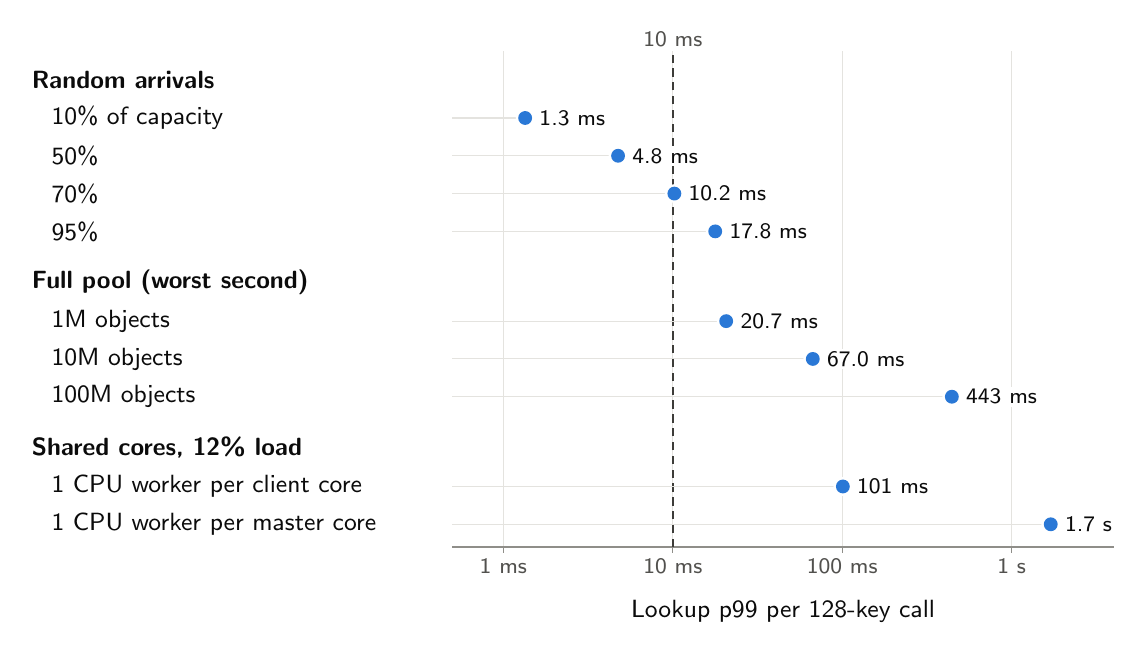
\begin{tikzpicture}[x=1cm,y=1cm]
\draw[draw=gridc, line width=0.4pt] (6.048,0.000) -- (6.048,6.300);
\draw[draw=axisc, line width=0.4pt] (6.048,0.000) -- (6.048,-0.070);
\node[tick, anchor=north] at (6.048,-0.090) {1 ms};
\draw[draw=gridc, line width=0.4pt] (8.200,0.000) -- (8.200,6.300);
\draw[draw=axisc, line width=0.4pt] (8.200,0.000) -- (8.200,-0.070);
\node[tick, anchor=north] at (8.200,-0.090) {10 ms};
\draw[draw=gridc, line width=0.4pt] (10.352,0.000) -- (10.352,6.300);
\draw[draw=axisc, line width=0.4pt] (10.352,0.000) -- (10.352,-0.070);
\node[tick, anchor=north] at (10.352,-0.090) {100 ms};
\draw[draw=gridc, line width=0.4pt] (12.504,0.000) -- (12.504,6.300);
\draw[draw=axisc, line width=0.4pt] (12.504,0.000) -- (12.504,-0.070);
\node[tick, anchor=north] at (12.504,-0.090) {1 s};
\draw[draw=axisc, line width=0.5pt] (5.400,0) -- (13.800,0);
\draw[ref] (8.200,0.000) -- (8.200,6.300);
\node[note, anchor=south] at (8.200,6.300) {10 ms};
\node[lab, anchor=west, font=\small\bfseries] at (0,5.940) {Random arrivals};
\node[lab, anchor=west] at (0.25,5.450) {10\% of capacity};
\draw[draw=gridc, line width=0.4pt] (5.400,5.450) -- (6.325,5.450);
\fill[white] (6.325,5.450) circle (3.4pt);
\fill[lookup] (6.325,5.450) circle (2.5pt);
\node[note, text=ink, anchor=west, fill=white, inner sep=1pt] at (6.465,5.450) {1.3 ms};
\node[lab, anchor=west] at (0.25,4.970) {50\%};
\draw[draw=gridc, line width=0.4pt] (5.400,4.970) -- (7.505,4.970);
\fill[white] (7.505,4.970) circle (3.4pt);
\fill[lookup] (7.505,4.970) circle (2.5pt);
\node[note, text=ink, anchor=west, fill=white, inner sep=1pt] at (7.645,4.970) {4.8 ms};
\node[lab, anchor=west] at (0.25,4.490) {70\%};
\draw[draw=gridc, line width=0.4pt] (5.400,4.490) -- (8.220,4.490);
\fill[white] (8.220,4.490) circle (3.4pt);
\fill[lookup] (8.220,4.490) circle (2.5pt);
\node[note, text=ink, anchor=west, fill=white, inner sep=1pt] at (8.360,4.490) {10.2 ms};
\node[lab, anchor=west] at (0.25,4.010) {95\%};
\draw[draw=gridc, line width=0.4pt] (5.400,4.010) -- (8.739,4.010);
\fill[white] (8.739,4.010) circle (3.4pt);
\fill[lookup] (8.739,4.010) circle (2.5pt);
\node[note, text=ink, anchor=west, fill=white, inner sep=1pt] at (8.879,4.010) {17.8 ms};
\node[lab, anchor=west, font=\small\bfseries] at (0,3.360) {Full pool (worst second)};
\node[lab, anchor=west] at (0.25,2.870) {1M objects};
\draw[draw=gridc, line width=0.4pt] (5.400,2.870) -- (8.878,2.870);
\fill[white] (8.878,2.870) circle (3.4pt);
\fill[lookup] (8.878,2.870) circle (2.5pt);
\node[note, text=ink, anchor=west, fill=white, inner sep=1pt] at (9.018,2.870) {20.7 ms};
\node[lab, anchor=west] at (0.25,2.390) {10M objects};
\draw[draw=gridc, line width=0.4pt] (5.400,2.390) -- (9.978,2.390);
\fill[white] (9.978,2.390) circle (3.4pt);
\fill[lookup] (9.978,2.390) circle (2.5pt);
\node[note, text=ink, anchor=west, fill=white, inner sep=1pt] at (10.118,2.390) {67.0 ms};
\node[lab, anchor=west] at (0.25,1.910) {100M objects};
\draw[draw=gridc, line width=0.4pt] (5.400,1.910) -- (11.744,1.910);
\fill[white] (11.744,1.910) circle (3.4pt);
\fill[lookup] (11.744,1.910) circle (2.5pt);
\node[note, text=ink, anchor=west, fill=white, inner sep=1pt] at (11.884,1.910) {443 ms};
\node[lab, anchor=west, font=\small\bfseries] at (0,1.260) {Shared cores, 12\% load};
\node[lab, anchor=west] at (0.25,0.770) {1 CPU worker per client core};
\draw[draw=gridc, line width=0.4pt] (5.400,0.770) -- (10.360,0.770);
\fill[white] (10.360,0.770) circle (3.4pt);
\fill[lookup] (10.360,0.770) circle (2.5pt);
\node[note, text=ink, anchor=west, fill=white, inner sep=1pt] at (10.500,0.770) {101 ms};
\node[lab, anchor=west] at (0.25,0.290) {1 CPU worker per master core};
\draw[draw=gridc, line width=0.4pt] (5.400,0.290) -- (13.000,0.290);
\fill[white] (13.000,0.290) circle (3.4pt);
\fill[lookup] (13.000,0.290) circle (2.5pt);
\node[note, text=ink, anchor=west, fill=white, inner sep=1pt] at (13.140,0.290) {1.7 s};
\node[lab, anchor=north] at (9.600,-0.62) {Lookup p99 per 128-key call};
\end{tikzpicture}}%
\pdfvariable horigin=0pt
\pdfvariable vorigin=0pt
\pagewidth=\dimexpr\wd0+8pt\relax
\pageheight=\dimexpr\ht0+\dp0+8pt\relax
\shipout\vbox{\kern4pt\hbox{\kern4pt\box0\kern4pt}\kern4pt}
\end{document}
